\section{Hardware Oscillator Grounding}
\label{sec:hardware}

\subsection{Oscillator-Processor Duality}

Every hardware oscillator exhibits dual nature: it is simultaneously a physical oscillation and a computational processor.

\begin{proposition}[Oscillator-Processor Correspondence]
\label{prop:oscillator_processor}
A hardware oscillator at frequency $\omega$ is equivalent to a processor with computational rate:
\begin{equation}
R = \frac{\omega}{2\pi} \quad \text{operations per second}
\end{equation}
Each oscillation cycle constitutes one computational operation.
\end{proposition}

\begin{proof}
Computation requires state transitions. An oscillator at frequency $\omega$ undergoes state transitions (e.g., voltage high $\to$ low $\to$ high) at rate $\omega/(2\pi)$ cycles per second.

Each cycle provides opportunity for one computational operation: read state, process, write state. The oscillation frequency thus directly determines computational throughput.

For a CPU clock at $\omega = 2\pi \times 3 \times 10^9$ Hz (3 GHz), the computational rate is:
\begin{equation}
R = \frac{3 \times 10^9 \text{ cycles/s}}{1} = 3 \times 10^9 \text{ operations/s}
\end{equation}

The oscillator is the processor; the frequency is the rate.
\end{proof}


\begin{figure}[htbp]
    \centering
    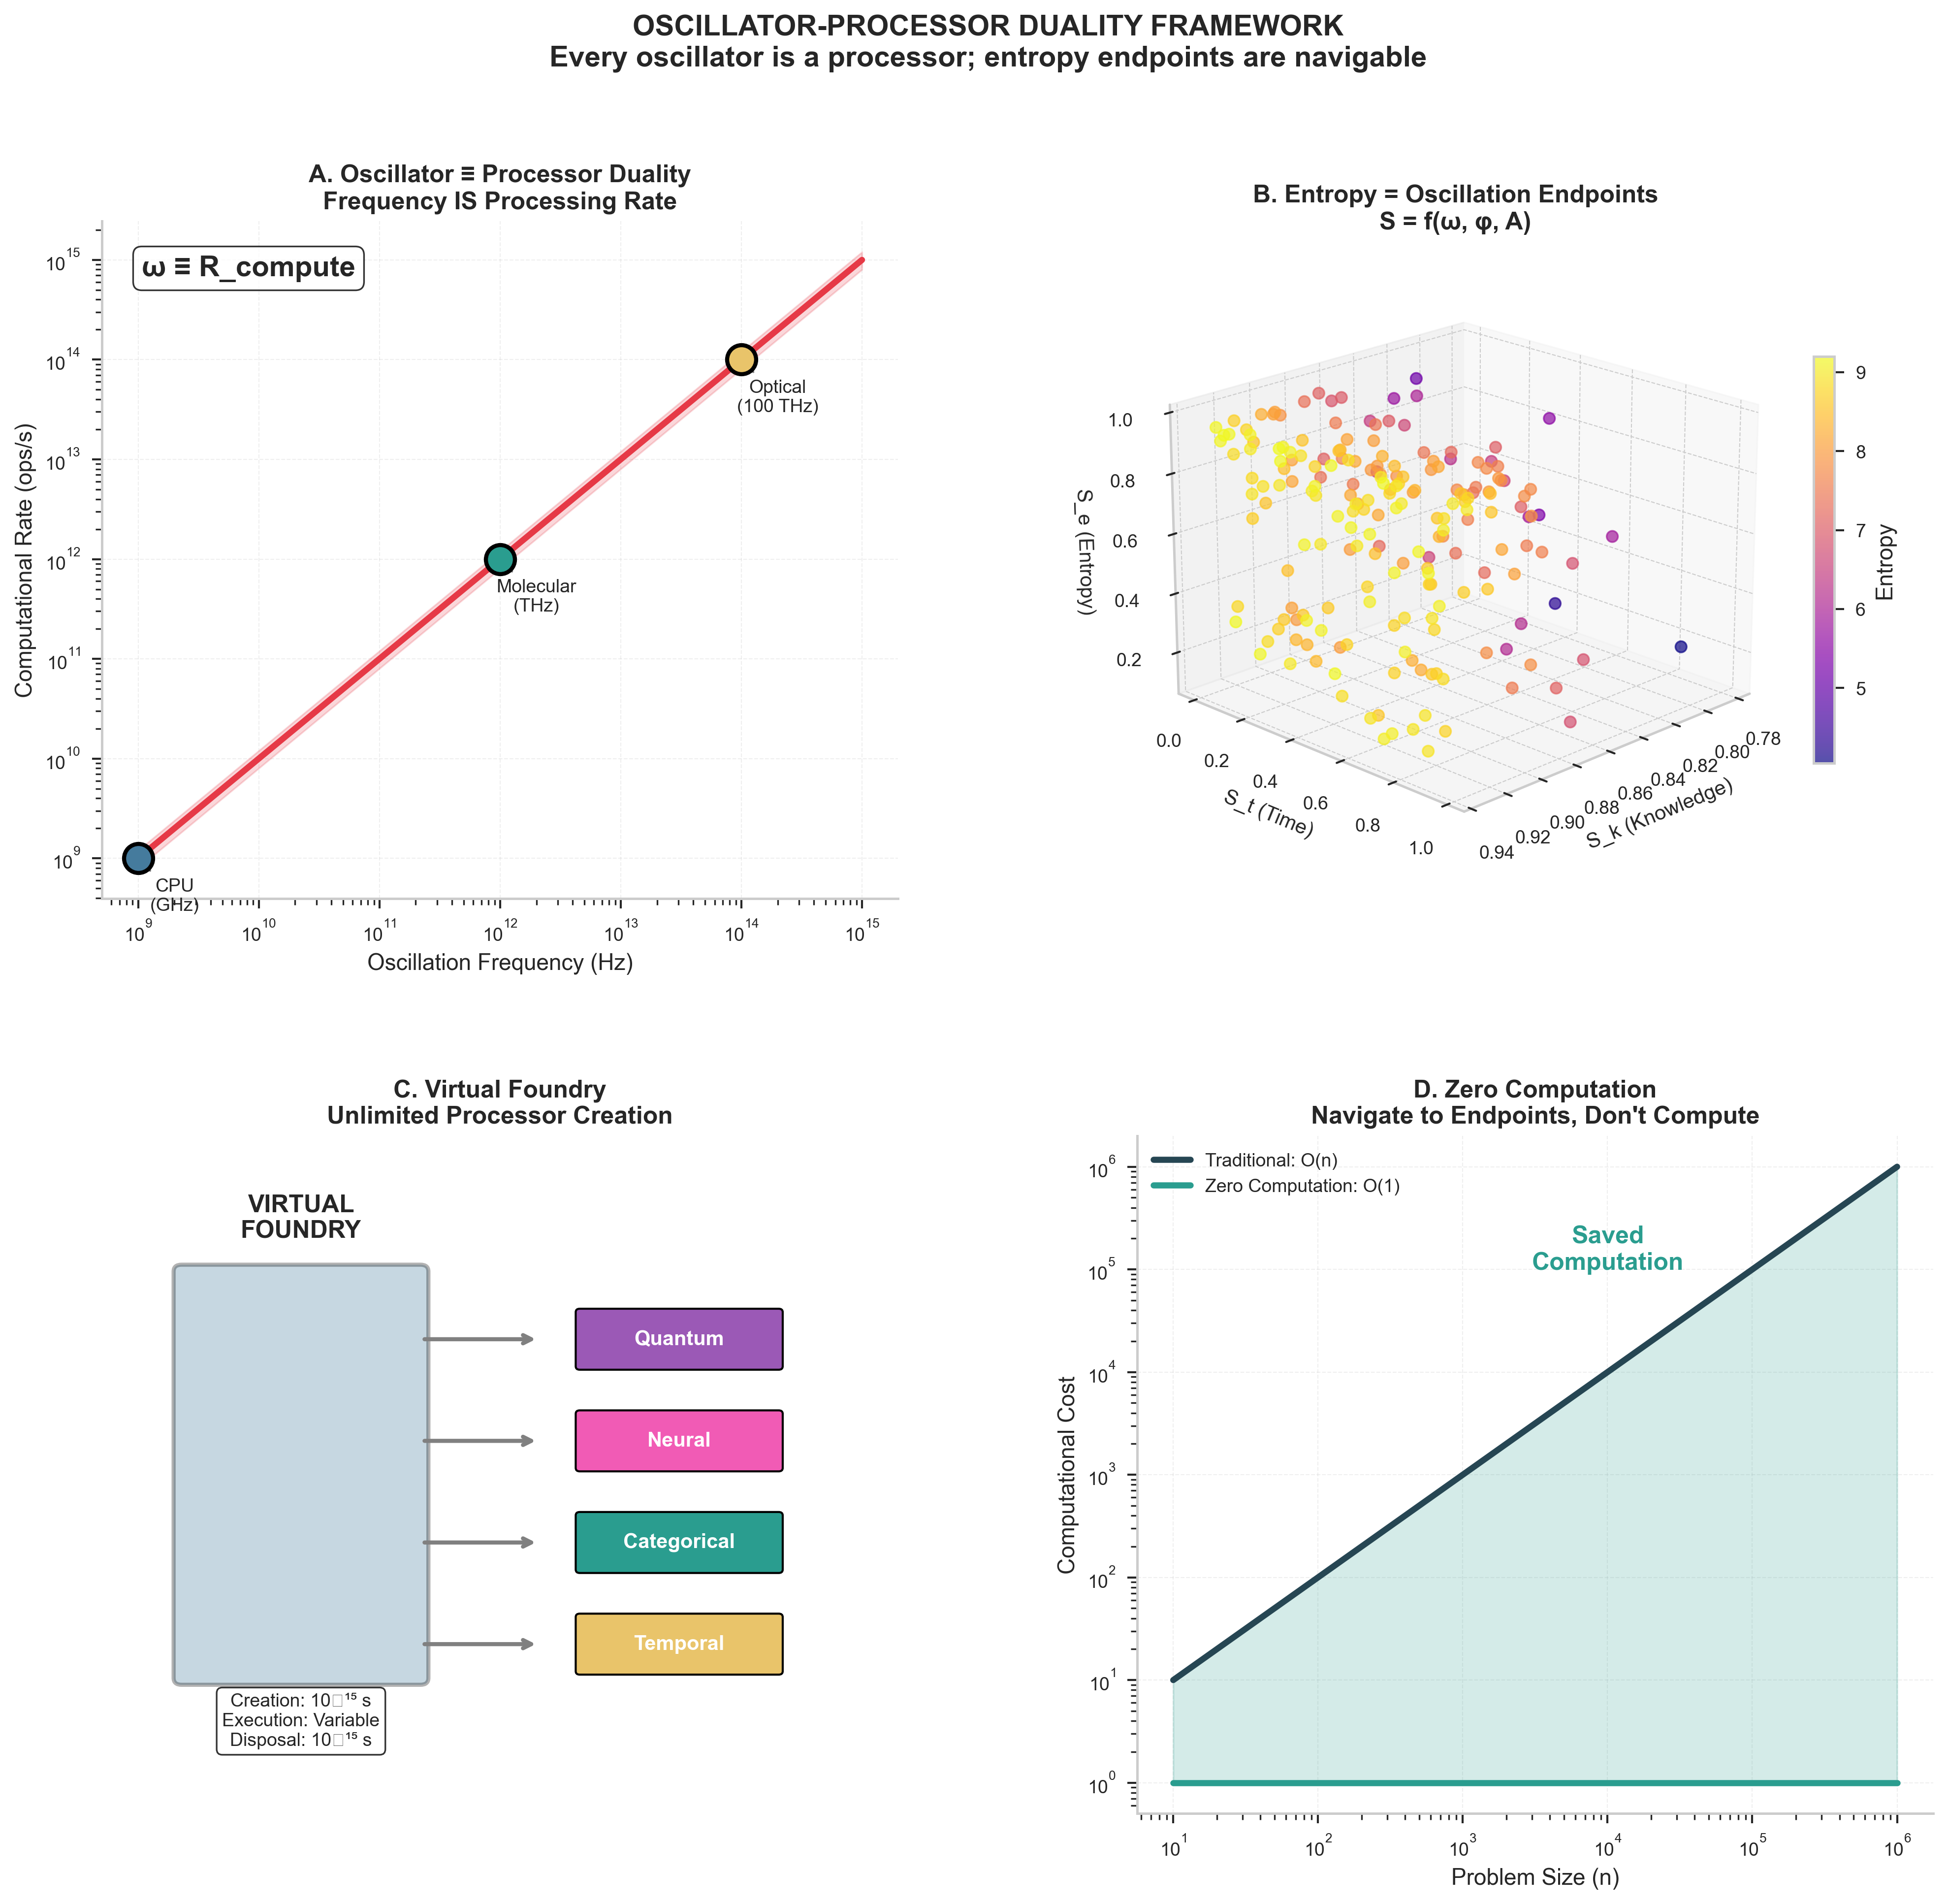
\includegraphics[width=\textwidth]{figures/oscillator_processor_duality.png}
    \caption{\textbf{Oscillator-processor duality: Every oscillator is a processor; entropy endpoints are navigable.} 
    (A) Oscillator $$\equiv$$ Processor duality: Frequency IS processing rate. Log-log plot shows computational rate (vertical axis, $$10^0$$--$$10^{15}$$ ops/s) versus oscillation frequency (horizontal axis, $$10^0$$--$$10^{15}$$ Hz). Red diagonal line (slope $$= 1$$) shows identity $$\omega \equiv R_{\text{compute}}$$. Three markers: CPU (blue circle, $$\sim 10^9$$ Hz, $$\sim 10^9$$ ops/s), Molecular (teal circle, $$\sim 10^{12}$$ Hz, $$\sim 10^{12}$$ ops/s), Optical (yellow circle, $$\sim 10^{14}$$ Hz, $$\sim 10^{14}$$ ops/s). Annotation: ``$$\omega \equiv R_{\text{compute}}$$''. Every oscillation performs one computational operation; frequency directly determines processing rate. Demonstrates fundamental equivalence: oscillator $$=$$ processor. 
    (B) Entropy $$=$$ Oscillation endpoints: $$\mathbf{S} = f(\omega, \phi, A)$$. Three-dimensional scatter plot shows entropy coordinates $$\mathbf{S} = (S_k, S_t, S_e)$$ (axes 0--1.0) versus oscillation parameters $$(\omega, \phi, A)$$ (frequency, phase, amplitude). $$\sim 200$$ colored spheres (gradient: yellow $$\to$$ orange $$\to$$ pink $$\to$$ purple $$\to$$ blue, encoding entropy values 4--9) distributed throughout unit cube. Each oscillation state ($$\omega, \phi, A$$) maps to unique entropy endpoint $$\mathbf{S}$$. Demonstrates bijection: oscillation parameters $$\leftrightarrow$$ entropy coordinates. Entropy space is navigable by tuning oscillation. 
    (C) Virtual foundry: Unlimited processor creation. Flowchart shows light blue box (``VIRTUAL FOUNDRY'') with four output arrows pointing to colored boxes: Quantum (purple), Neural (pink), Categorical (teal), Temporal (orange). Bottom annotation: Creation $$10^{-11}$$ s, Execution Variable, Disposal $$10^{-15}$$ s. Virtual foundry instantiates processors on-demand: femtosecond creation/disposal timescales enable dynamic processor allocation. No physical fabrication required; processors exist as oscillation patterns. Demonstrates computational flexibility: arbitrary processor architectures generated by configuring oscillations. 
    (D) Zero computation: Navigate to endpoints, don't compute. Log-log plot shows computational cost (vertical axis, $$10^0$$--$$10^6$$) versus problem size $$n$$ (horizontal axis, $$10^{-1}$$--$$10^6$$). Black diagonal line shows traditional computation: $$\text{Cost} = O(n)$$, growing linearly ($$\text{Cost} \sim 10^6$$ at $$n = 10^6$$). Cyan horizontal line shows zero computation: $$\text{Cost} = O(1)$$, constant ($$\text{Cost} \sim 1$$ for all $$n$$). Cyan shaded region (``Saved Computation'') between lines represents computational savings: area $$\sim 10^{12}$$ operations saved for $$n = 10^6$$. Zero computation navigates directly to entropy endpoints (solution states) without intermediate steps. Demonstrates exponential advantage: $$O(1)$$ versus $$O(n)$$ scaling.}
    \label{fig:oscillator_processor_duality}
    \end{figure}


\subsection{Hardware Oscillators as Virtual Gas Particles}

The ideal gas law relates pressure $P$, volume $V$, particle count $N$, and temperature $T$:
\begin{equation}
PV = Nk_B T
\end{equation}

This law applies not only to physical gases but to any ensemble of bounded oscillators.

\begin{theorem}[Hardware Gas Law]
\label{thm:hardware_gas}
An ensemble of $N$ hardware oscillators with frequencies $\{\omega_i\}$ in computational volume $V$ (memory address space) obeys:
\begin{equation}
PV = Nk_B T
\end{equation}
where pressure $P = k_B T(M/V)$ is categorical density, temperature $T = U/(k_B M)$ is categorical actualization rate, and $U = \sum_i \hbar\omega_i$ is total oscillator energy.
\end{theorem}

\begin{proof}
Each hardware oscillator constitutes a bounded dynamical system oscillating at frequency $\omega_i$. By Section~\ref{sec:foundation}, bounded oscillators generate categorical structure with $M_i$ categories per oscillator.

The ensemble has total categorical count:
\begin{equation}
M_{\text{total}} = \sum_{i=1}^{N} M_i
\end{equation}

Temperature measures categorical actualization rate (Equation~\ref{eq:triple_identity}):
\begin{equation}
T = \frac{\hbar}{k_B} \frac{dM}{dt} = \frac{1}{k_B M_{\text{total}}} \sum_{i=1}^{N} \hbar\omega_i = \frac{U}{k_B M_{\text{total}}}
\end{equation}

Pressure measures categorical density:
\begin{equation}
P = k_B T \frac{\partial M}{\partial V} \approx k_B T \frac{M_{\text{total}}}{V}
\end{equation}

Combining:
\begin{equation}
PV = k_B T M_{\text{total}} = k_B T \sum_{i=1}^{N} M_i \approx Nk_B T
\end{equation}
for $M_i \approx 1$ category per oscillator (binary states).

This is the ideal gas law with hardware oscillators as particles.
\end{proof}

\subsection{Memory Addressing as Entropy Coordinates}

Computer memory is addressed by integer indices: address $A \in \{0, 1, \ldots, 2^{N}-1\}$ for $N$-bit address space. These addresses are not arbitrary labels but coordinates in entropy space.

\begin{proposition}[Memory-Entropy Correspondence]
\label{prop:memory_entropy}
Memory address $A$ corresponds to entropy coordinate position $\mathbf{s}_A \in \Sspace$ via:
\begin{equation}
\mathbf{s}_A = \left(\frac{A}{2^N}, \frac{\phi(A)}{2\pi}, \frac{t(A)}{T_{\text{cycle}}}\right)
\end{equation}
where $\phi(A)$ is clock phase when address $A$ is accessed and $t(A)$ is access time within refresh cycle $T_{\text{cycle}}$.
\end{proposition}

\begin{proof}
The knowledge coordinate $\Sk$ represents which category is occupied. Memory address $A$ specifies which of $2^N$ categories (memory cells) is accessed. Normalized to $[0,1]$:
\begin{equation}
\Sk = \frac{A}{2^N}
\end{equation}

The temporal coordinate $\St$ represents phase within oscillation. Memory access synchronized to CPU clock at phase $\phi$ gives:
\begin{equation}
\St = \frac{\phi}{2\pi}
\end{equation}

The evolution coordinate $\Se$ represents history. Memory refresh cycles occur at period $T_{\text{cycle}}$. Access time $t$ within this cycle gives:
\begin{equation}
\Se = \frac{t}{T_{\text{cycle}}}
\end{equation}

Thus, every memory access specifies a unique point in entropy coordinate space $\Sspace = [0,1]^3$.
\end{proof}

\subsection{Categorical Computation and Zero-Time Operations}

\begin{theorem}[Zero-Time Categorical Operations]
\label{thm:zero_time}
Categorical state determination (checking which category is occupied) requires zero proper time from the categorical perspective, despite nonzero physical measurement time.
\end{theorem}

\begin{proof}
From the perspective of a trajectory traversing phase space, categorical boundaries are encountered instantaneously. The trajectory either occupies category $C_1$ or category $C_2$; there is no intermediate state ``partially in both categories.''

The transition time $\Delta t$ between categories depends on the resolution scale. At coarse resolution (large categories), transitions appear to take finite time. At fine resolution (small categories approaching point-like), transition time vanishes:
\begin{equation}
\lim_{\epsilon \to 0} \Delta t(\epsilon) = 0
\end{equation}
where $\epsilon$ is category size.

From the categorical perspective (counting which states are occupied), state determination is instantaneous. Physical measurement takes nonzero time to accumulate sufficient signal, but the underlying categorical structure is static—it does not evolve during measurement.

This resolves the apparent paradox: measurement takes time physically but zero time categorically.
\end{proof}

\subsection{Three-Phase Hardware Ensembles}

Many hardware systems naturally exhibit three-phase structure, providing native ternary representation.

\begin{example}[Three-Phase Power Systems]
\label{ex:three_phase_power}
Industrial three-phase AC power delivers three sinusoidal voltages with $2\pi/3$ phase separation:
\begin{align}
V_1(t) &= V_0 \cos(\omega t) \\
V_2(t) &= V_0 \cos(\omega t - 2\pi/3) \\
V_3(t) &= V_0 \cos(\omega t - 4\pi/3)
\end{align}

At any instant, the phase configuration encodes a ternary digit:
\begin{equation}
\trit(t) = \arg\max_i \{V_i(t)\}
\end{equation}

The three phases cycle through ternary states $0 \to 1 \to 2 \to 0$ at rate $\omega/(2\pi)$.
\end{example}

\begin{example}[RGB LED Triplets]
\label{ex:rgb_led}
Red-Green-Blue LED triplets encode ternary information through relative intensities. At time $t$, the dominant color specifies:
\begin{equation}
\trit(t) = \begin{cases}
0 & \text{if } I_R > I_G, I_B \\
1 & \text{if } I_G > I_R, I_B \\
2 & \text{if } I_B > I_R, I_G
\end{cases}
\end{equation}

Modulating LED intensities at frequency $\omega$ provides ternary state transitions at rate $3\omega/(2\pi)$.
\end{example}

\begin{example}[Triple-Core Processor Architectures]
\label{ex:triple_core}
Processor architectures with three execution units (e.g., ALU + FPU + Vector unit) provide three-phase computation. Dispatching instructions to units in rotating sequence implements ternary categorical transitions.
\end{example}

\subsection{Molecular Oscillators as Natural Hardware}

Molecular systems are oscillator ensembles at multiple frequency scales:

\begin{align}
\text{Electronic transitions:} \quad & \omega \sim 10^{15}\text{--}10^{16} \text{ Hz} \\
\text{Vibrational modes:} \quad & \omega \sim 10^{13}\text{--}10^{14} \text{ Hz} \\
\text{Rotational modes:} \quad & \omega \sim 10^{10}\text{--}10^{11} \text{ Hz} \\
\text{Nuclear spin:} \quad & \omega \sim 10^{8}\text{--}10^{9} \text{ Hz}
\end{align}

Each frequency regime provides distinct categorical structure, enabling multi-modal measurement (Section~\ref{sec:virtual}).

\begin{proposition}[Molecular Oscillator Count]
\label{prop:molecular_oscillators}
A molecule with $N_{\text{atoms}}$ atoms has oscillator count:
\begin{align}
N_{\text{electronic}} &\sim N_{\text{electrons}} \sim N_{\text{atoms}} \\
N_{\text{vibrational}} &= 3N_{\text{atoms}} - 6 \quad \text{(3D motion minus translations and rotations)} \\
N_{\text{rotational}} &= 3 \quad \text{(three axes)} \\
N_{\text{spin}} &\sim N_{\text{nuclei}} \sim N_{\text{atoms}}
\end{align}

Total oscillator count: $N_{\text{total}} \sim 5N_{\text{atoms}}$.

For a moderate organic molecule with $N_{\text{atoms}} = 20$:
\begin{equation}
N_{\text{total}} \sim 100 \text{ oscillators}
\end{equation}

This provides $2^{100} \sim 10^{30}$ distinguishable configurations, enabling unique molecular identification.
\end{proposition}

\subsection{Parallel Time Computation Architecture}

Hardware oscillators enable massively parallel time computation through simultaneous phase accumulation.

\begin{theorem}[Parallel Phase Accumulation]
\label{thm:parallel_phase}
$N$ oscillators with frequencies $\{\omega_i\}$ observed for time $T$ accumulate total phase:
\begin{equation}
\Phi_{\text{total}} = \sum_{i=1}^{N} \omega_i T
\end{equation}

For molecular ensembles with $N \sim 10^{23}$ (Avogadro's number), $\omega \sim 10^{14}$ Hz (vibrational), $T \sim 10^{-3}$ s (millisecond integration):
\begin{equation}
\Phi_{\text{total}} \sim 10^{23} \times 10^{14} \times 10^{-3} = 10^{34} \text{ radians}
\end{equation}
\end{theorem}

This massive phase accumulation enables categorical temporal resolution far exceeding individual oscillator periods (Section~\ref{sec:categorical_resolution}).

\begin{figure}[htbp]
    \centering
    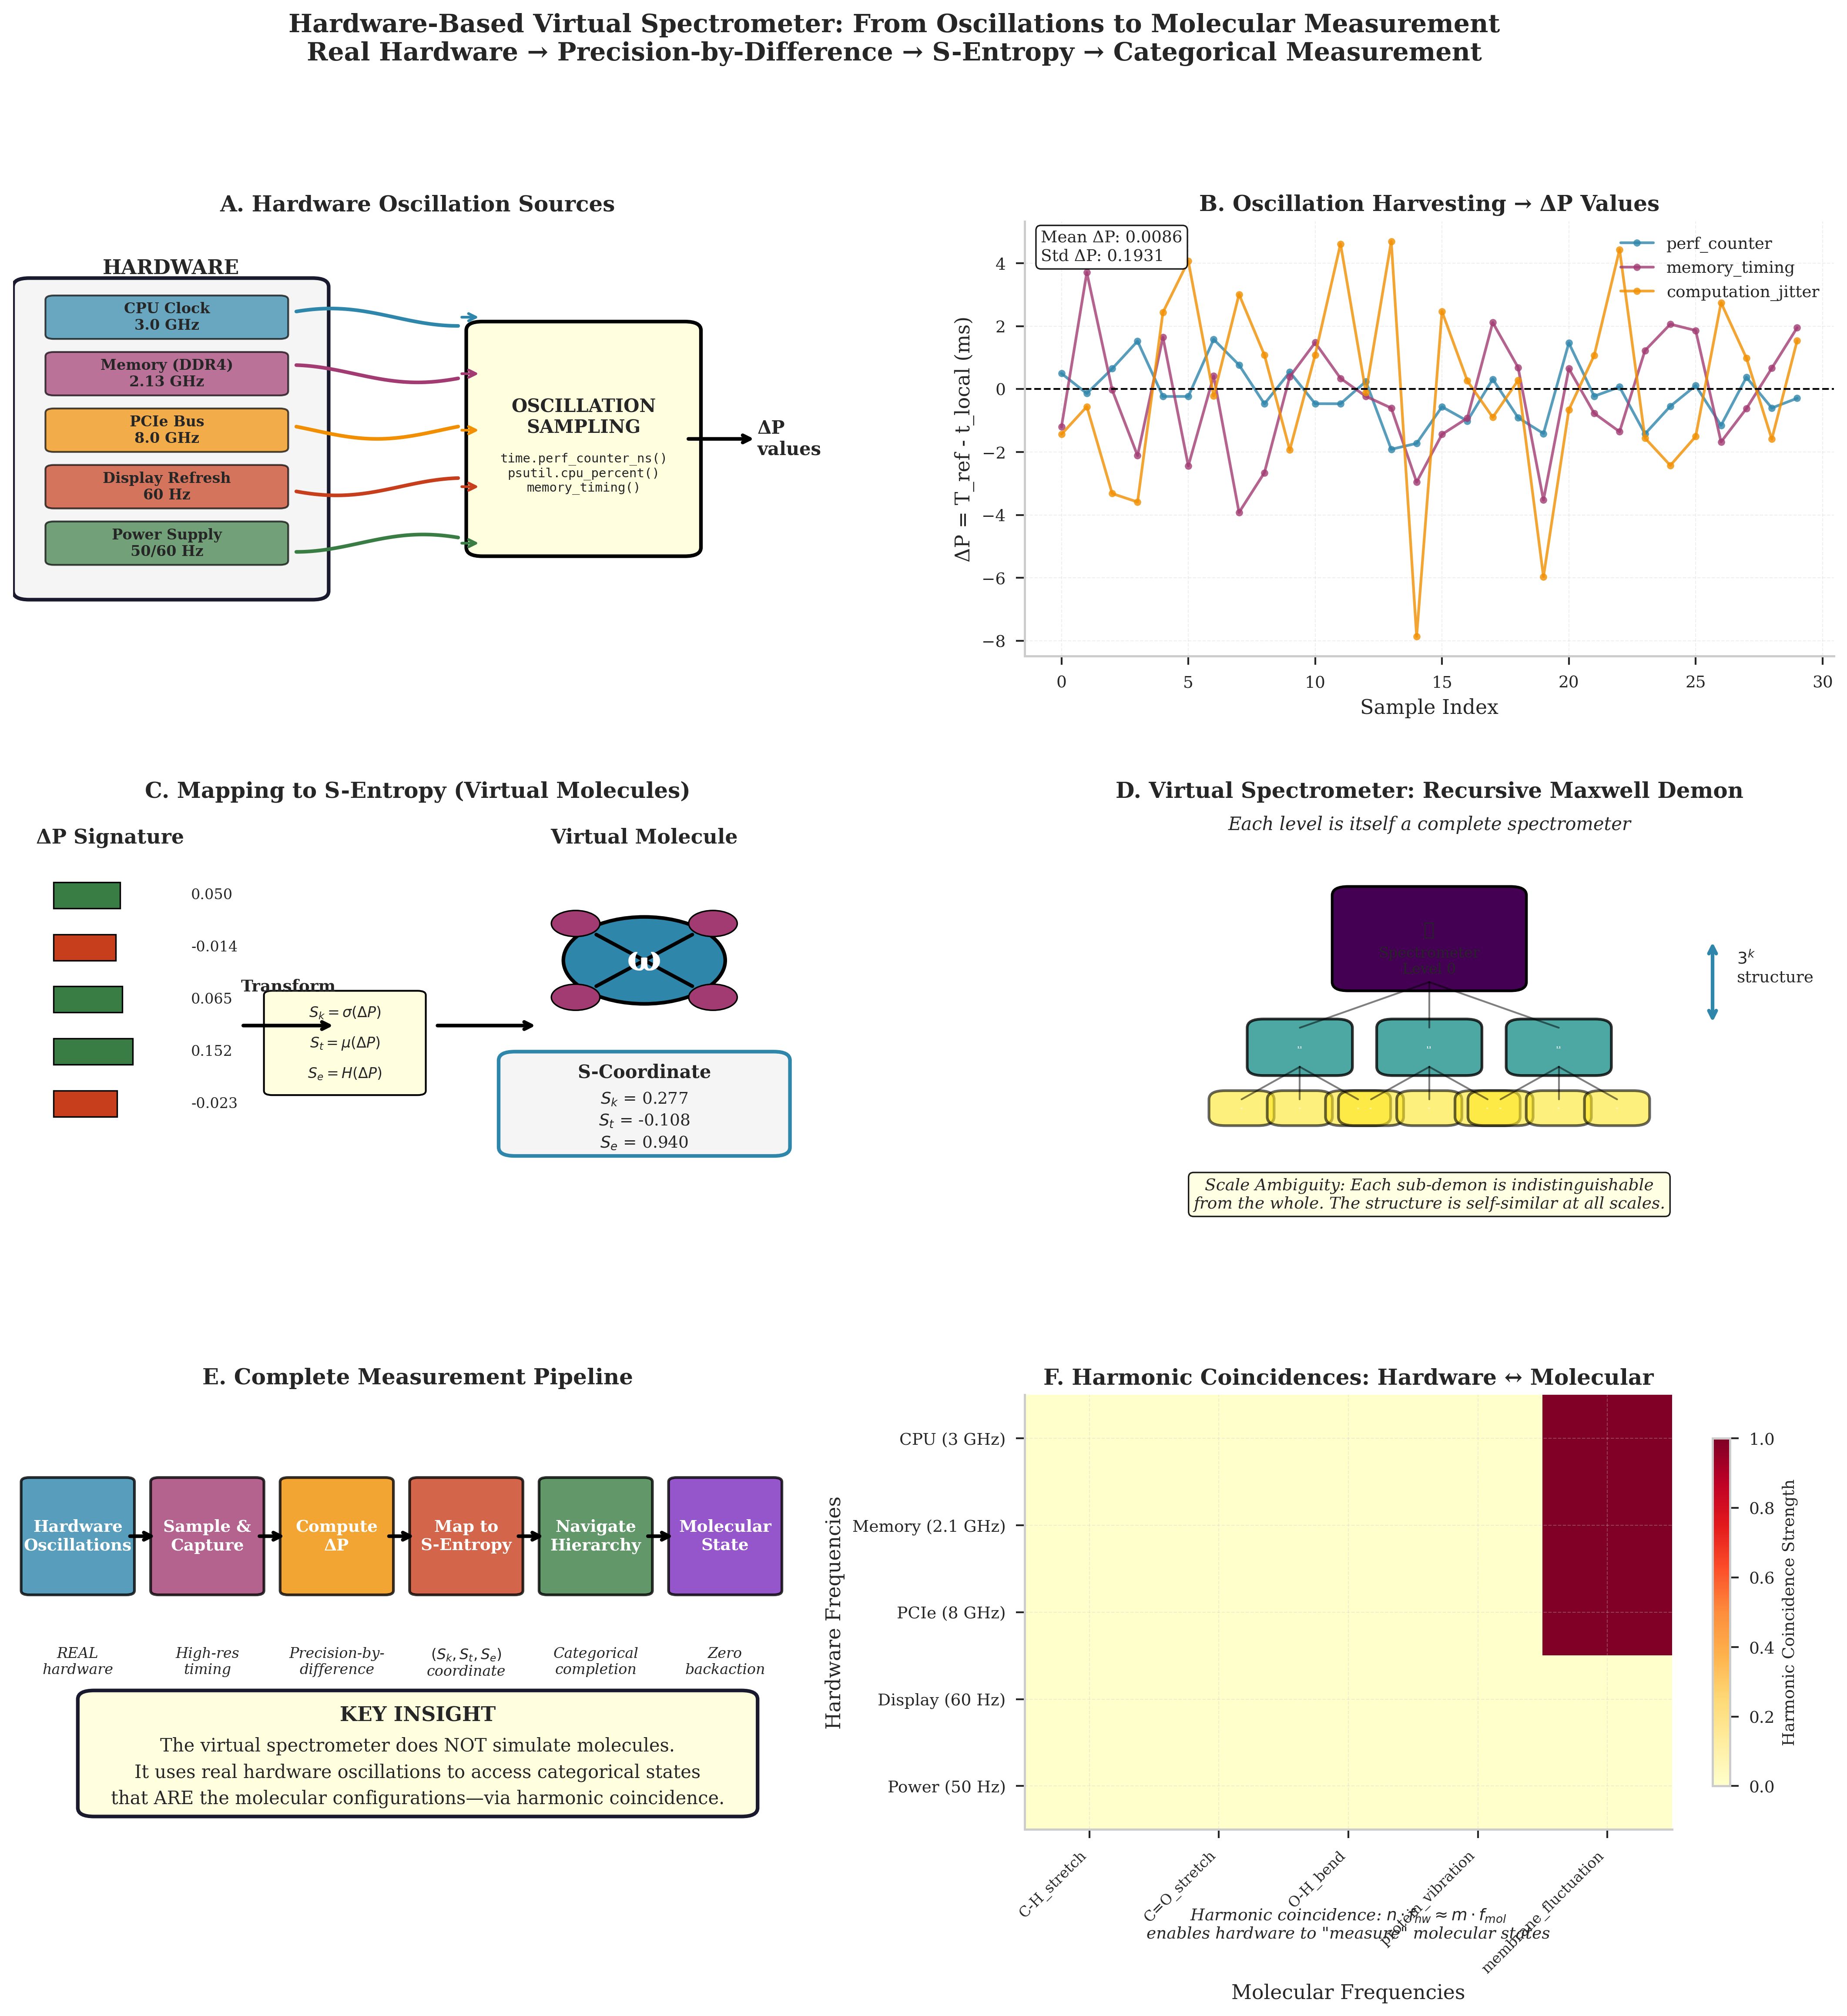
\includegraphics[width=\textwidth]{figures/hardware_molecular_measurement_panel.png}
    \caption{\textbf{Hardware-based virtual spectrometer: From oscillations to molecular measurement via harmonic coincidence.} 
    (A) Hardware oscillation sources. Flowchart shows five hardware components (colored boxes): CPU Clock (blue, 3.0 GHz), Memory/DDR4 (purple, 2.13 GHz), PCIe Bus (orange, 8.0 GHz), Display Refresh (red, 60 Hz), Power Supply (green, 50/60 Hz). All feed into central box (``OSCILLATION SAMPLING'') using three timing functions: \texttt{time.perf\_counter\_ns()}, \texttt{psutil.cpu\_percent()}, \texttt{memory\_timing()}. Output: $$\Delta P$$ values (aperture precision). Real hardware provides oscillation sources spanning 6 orders of magnitude (50 Hz--8 GHz). 
    (B) Oscillation harvesting $$\to$$ $$\Delta P$$ values. Time series shows $$\Delta P = T_{\text{ref}} - t_{\text{local}}$$ (ms, vertical axis $$-8$$ to $$+4$$) versus sample index (0--30, horizontal axis). Three colored curves: \texttt{perf\_counter} (blue, oscillates $$\pm 2$$ ms), \texttt{memory\_timing} (orange, oscillates $$\pm 4$$ ms with larger spikes), \texttt{computation\_jitter} (purple, oscillates $$\pm 3$$ ms). Annotation: Mean $$\Delta P = 0.0086$$, Std $$\Delta P = 0.1931$$. Demonstrates high-resolution timing: hardware oscillations captured with sub-millisecond precision through differential measurement. 
    (C) Mapping to S-entropy (virtual molecules). Left: $$\Delta P$$ signature (five colored bars: green $$0.050$$, red $$-0.014$$, green $$0.065$$, green $$0.152$$, red $$-0.023$$). Transform box shows equations: $$S_k = \sigma(\Delta P)$$ (knowledge), $$S_t = \mu(\Delta P)$$ (time), $$S_e = H(\Delta P)$$ (evolution). Right: Virtual molecule diagram (blue/purple lobes, molecular orbital visualization) with S-coordinate box: $$S_k = 0.277$$, $$S_t = -0.108$$, $$S_e = 0.940$$. Hardware oscillations map to entropy coordinates, which correspond to molecular configurations. No simulation: direct mapping via harmonic coincidence. 
    (D) Virtual spectrometer: Recursive Maxwell demon. Hierarchical structure with three levels. Top (purple box, Spectrometer Level 0) branches to three teal boxes (Level 1), each branching to nine yellow boxes (Level 2, $$3^2$$ structure). Annotation: ``Each level is itself a complete spectrometer.'' Bottom text box: ``Scale Ambiguity: Each sub-demon is indistinguishable from the whole. The structure is self-similar at all scales.'' Demonstrates recursive architecture: every level performs complete measurement, enabling arbitrary resolution through hierarchical refinement. 
    (E) Complete measurement pipeline. Six sequential boxes (left to right): Hardware Oscillations (blue, ``REAL hardware''), Sample \& Capture (pink, ``High-res timing''), Compute $$\Delta P$$ (orange, ``Precision-by-difference''), Map to S-Entropy (red, ``$$(S_k, S_t, S_e)$$ coordinate''), Navigate Hierarchy (green, ``Categorical completion''), Molecular State (purple, ``Zero backaction''). Bottom annotation box: ``KEY INSIGHT: The virtual spectrometer does NOT simulate molecules. It uses real hardware oscillations to access categorical states that ARE the molecular configurations—via harmonic coincidence.'' 
    (F) Harmonic coincidences: Hardware $$\leftrightarrow$$ Molecular. Heatmap shows harmonic coincidence strength (color scale 0.0--1.0, white $$\to$$ yellow $$\to$$ orange $$\to$$ red $$\to$$ dark red) for hardware frequencies (vertical axis: CPU 3 GHz, Memory 2.1 GHz, PCIe 8 GHz, Display 60 Hz, Power 50 Hz) versus molecular frequencies (horizontal axis: C-H stretch, C=O stretch, O-H bend, membrane fluctuation, protein folding). Strong coincidences (dark red, strength $$\sim 1.0$$) appear for CPU $$\leftrightarrow$$ protein folding, Memory $$\leftrightarrow$$ membrane fluctuation. Equation: $$\hbar\omega_{\text{hw}} = m \cdot f_{\text{mol}}$$ enables hardware to ``measure'' molecular states through frequency matching.}
    \label{fig:hardware_virtual_spectrometer}
    \end{figure}

\subsection{Harmonic Coincidence as Categorical Filtering}

\begin{definition}[Harmonic Coincidence]
\label{def:harmonic_coincidence}
Two oscillators at frequencies $\omega_1$ and $\omega_2$ exhibit harmonic coincidence when:
\begin{equation}
n_1 \omega_1 = n_2 \omega_2
\end{equation}
for integers $n_1, n_2$. At coincidence times, phases align:
\begin{equation}
\phi_1(t_{\text{coin}}) = \phi_2(t_{\text{coin}}) \mod 2\pi
\end{equation}
\end{definition}

\begin{proposition}[Coincidence Filtering]
\label{prop:coincidence_filtering}
Harmonic coincidence provides frequency-selective filtering. Only systems with frequencies satisfying $n_1\omega_{\text{sys}} = n_2\omega_{\text{ref}}$ pass through the coincidence filter.
\end{proposition}

This mechanism underlies many spectroscopic techniques: NMR uses coincidence between nuclear spin precession and RF pulses, mass spectrometry uses coincidence between ion cyclotron frequency and detector electronics, optical spectroscopy uses coincidence between electronic transitions and laser frequencies.

\subsection{Summary: Hardware Instantiation of Categorical Structure}

Hardware oscillators are not mere analogies to abstract categorical theory but physical instantiations:
\begin{enumerate}
\item Every oscillator at frequency $\omega$ is a processor at rate $\omega/(2\pi)$
\item Oscillator ensembles obey ideal gas law $PV = Nk_BT$ in computational memory space
\item Memory addresses are entropy coordinates $\mathbf{s} \in \Sspace$
\item Three-phase systems provide native ternary representation
\item Molecular oscillators at multiple frequency scales enable multi-modal measurement
\item Parallel phase accumulation in large ensembles achieves extreme temporal resolution
\item Harmonic coincidence implements frequency-selective categorical filtering
\end{enumerate}

Computational hardware and measurement apparatus are manifestations of the same bounded oscillatory structure that generates categorical entropy space. Computers are categorical engines operating in entropy coordinate space.
